\chapter{Grundlagen}


\section{Subdivison Übersicht}

Subdivison Algorithmen erzeugen aus einem Ausgangspolygonnetz eine glatte Fläche.
Die glatte Zielfläche ist dabei der Grenzwert eines unendlichen, rekursiven Verfeinerungsschemas.
Abbildung~\ref{fig:sd} visualisiert die Anwendung eines Subdivison Algorithmus auf eine Kurve und auf eine Fläche.
Nach mehrfacher Anwendung der Unterteilung konvergiert die Kurve oder Fläche gegen die glatte Zielkurve bzw. Zielflähe.
\begin{figure}[h]
  \caption{Subdivison Algorithmus - Kurve und Fläche}
  \centering
  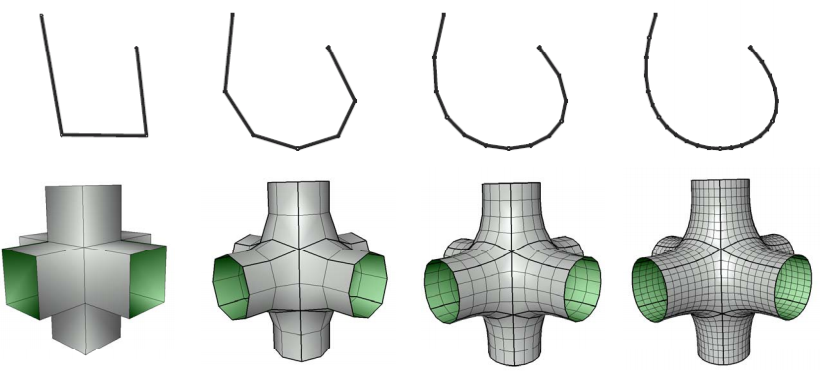
\includegraphics[width=0.8\textwidth]{content/media/sd.png}
  \\Quelle: \cite{Standford.24.07.2015}
  \label{fig:sd}
\end{figure}

Subdivision Algorithmen kann man anhand ihrer Eigenschaften Kategorisieren.
Ein Unterscheidungskriterium betriefft die Art und Weiße, wie unterteilt wird.
Man unterscheidet dabei zwischen \emph{Primal} und \emph{Dual}.
\begin{description}
 \item[Primal] Bei dieser Strategie wird die Oberfläche unterteilt ("face slit").
 Abbildung~\ref{fig:sd_primal} stellt diese Methode für ein Dreicksnetz und ein Vierecksnetz dar.
 \item[Dual] Auf der anderen Seite ist es möglich Eckpunkte in mehrere Eckpunkte aufzusplitten ("vertex split").
 Diese Methode ist in Abbildung~\ref{fig:sd_dual} abgebildet.
\end{description}
\begin{figure}[h]
  \caption{Primal (Face Split)}
  \centering
  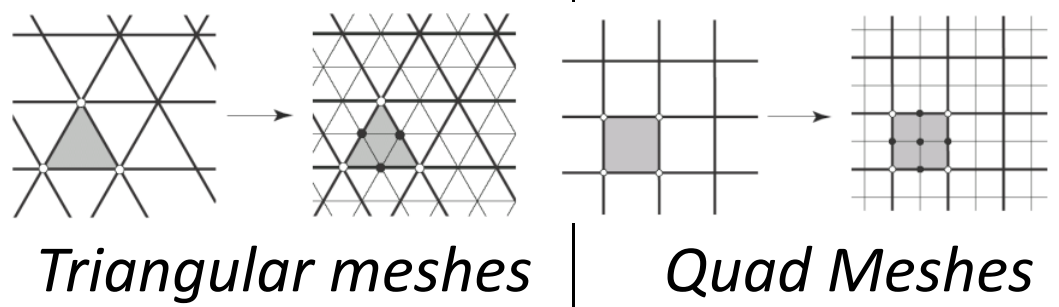
\includegraphics[width=0.7\textwidth]{content/media/sd_primal}
  \\Quelle: \cite{Standford.24.07.2015}
  \label{fig:sd_primal}
\end{figure}
\begin{figure}[h]
  \caption{Dual (Vertex Split)}
  \centering
  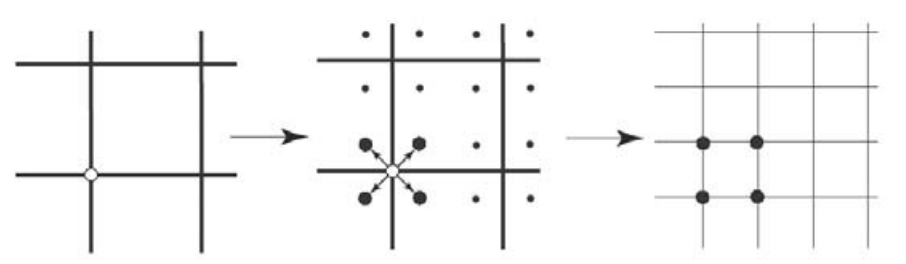
\includegraphics[width=0.7\textwidth]{content/media/sd_dual}
  \\Quelle: \cite{Standford.24.07.2015}
  \label{fig:sd_dual}
\end{figure}

Ein weiteres wesentliches Merkmal ist, ob Kontrollpunkte interpoliert werden oder nicht. 
\begin{description}
 \item[Approximation] Kontrollpunkte werden nicht interpoliert.
 \item[Interpolation] Kontrollpunkte werden interpoliert.
\end{description}

Tabelle~\ref{tab:sd_comp} listet die bekanntesten Subdivison Algorithmen auf und ordnet diese den Kategorien zu.
Zu jedem Algorithmus ist zusätzlich die "Glattheit" der Oberfläche angegeben (C-Stetigkeit).
Dies kann auch als Maß über die Qualität des Subdivision Algorithmus fungieren.
\begin{table}[h]
\caption{Subdivison Zoo}
\center
\begin{tabular}{|l|c|c|c}
\toprule
\multicolumn{3}{c|}{\textbf{Primal}} & \textbf{Dual}\\
\midrule
& \textbf{Dreiecksnetz} & \textbf{Vierecksnetz} & \\
\midrule
\textbf{Approximation} & Loop \((C^2)\) & Catmull-Clark \((C^2)\) & Doo-Sabin \((C^1)\) \\
\textbf{Interpolation} & Butterfly \((C^1)\) & Kobbelt \((C^1)\) & Biquartic \((C^2)\) \\
\bottomrule
\end{tabular}
\label{tab:sd_comp}
\end{table}

Abbildung~\ref{fig:sd_comp} Vergleicht die vier unterschiedlichen Subdivison Algorithmen Catmull-Clark, Loop, Doo-Sabin und Butterfly.
Man erkennt deutlich den interpolierenden Subdivison Algorithmus (Butterfly),
da dieser durch die harten Interpolationsbedingungen im Vergleich zu den approximierenden Algorithmen viel welligere ist.
\begin{figure}[h]
  \caption{Vergleich der Subdivison Algorithmen}
  \centering
  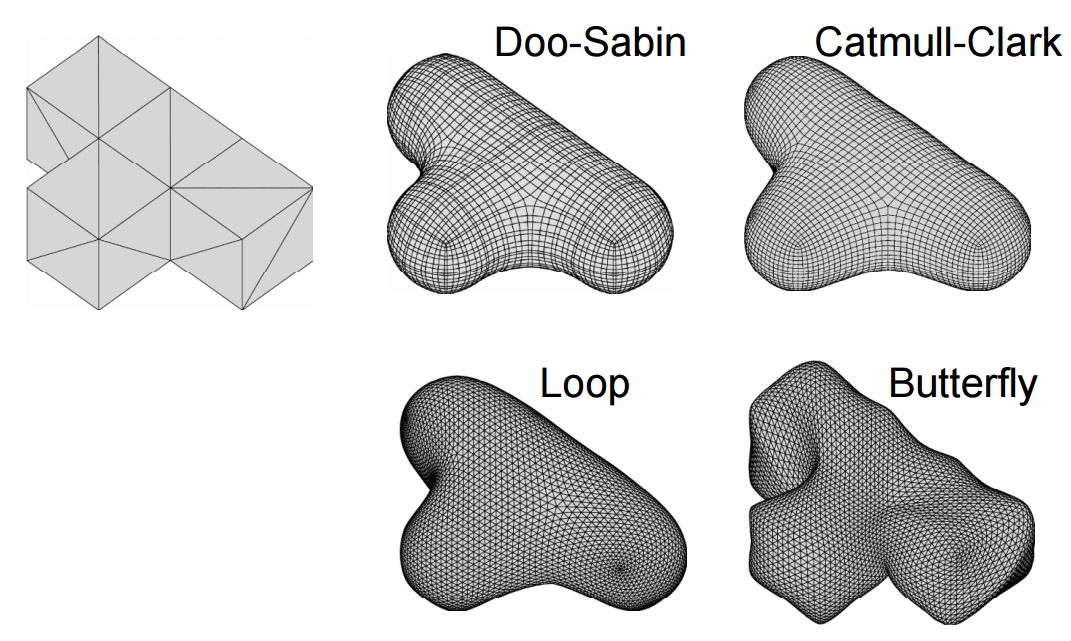
\includegraphics[width=0.9\textwidth]{content/media/sd_overview.png}
  \\Quelle: \cite{Standford.24.07.2015}
  \label{fig:sd_comp}
\end{figure}

\section{Auswahl der Subdivison Algorithmen}

Für das Projekt sollen folgende Algorithmen implementiert werden:
\begin{itemize}
	\item Catmull-Clark
	\item Loop
	\item Doo-Sabin
	\item Butterfly
\end{itemize}


